              %*****************************************%
              %                                         %
              % Template standard per la Tesi di Laurea %
              %            di Stefano Bianchi           %
              %                                         %
              %         versione: 27 marzo 2014         %
              %                                         %
              %   Updated and translated into English   %
              %             by Tommaso Fonda            %
              %                                         %
              %         revision: 6th Nov. 2023         %
              %                                         %
              %*****************************************%
              
% TexStudio special comment needed to make compile the template:
% 	1. Modify the compile command only for this file
%	2. Command to make work "minted" package
% !TeX document-id = {e97c24a0-e629-41ae-a1dd-cd418cd4f0c5}
% !TeX TXS-program:compile = txs:///pdflatex/[--shell-escape]

% Replace 'oneside' with 'twoside' for double-side printing
\documentclass[a4paper,12pt,oneside,openany]{book}

%*******************************************************
% Packages
%*******************************************************

% Typographical rules for the English language
\usepackage[english]{babel}

% Font-related packages
\usepackage[utf8]{inputenc}
\usepackage[T1]{fontenc}
\usepackage{inconsolata}

% ArteLatex suggestion
\usepackage{microtype}    % Better fonts
\usepackage{indentfirst}  % Indent first row of paragraph as used to do in Italian

% Needed to render the cover
\usepackage{fancyhdr}

% To draw graphs
\usepackage{tikz}
\usetikzlibrary{arrows.meta,decorations.pathmorphing,backgrounds,positioning,fit,petri}  % libraries to draw graphs
\tikzset{>=latex}  % fancy arrows

% Figures and subfigures
%\usepackage{graphicx}  % Removed since already loaded by tikz
\usepackage{subfig}

% Improved tables
\usepackage{tabularx}
\usepackage{longtable}

% Table according to ArteLatex
\usepackage{caption}
\captionsetup{tableposition=top, figureposition=bottom, font=small, format=hang, labelfont={sf,bf}}
\usepackage{booktabs}
\usepackage{multirow}

% To have appendices appear in the TOC
\usepackage[titletoc]{appendix}

% Needed for floating images
\usepackage{float}

% Improved verbatim appearance
\usepackage{fancyvrb}

% Math stuff
\usepackage{amsmath}
\numberwithin{equation}{section}
\usepackage{amsfonts}
\newcommand{\numberset}{\mathbb}  % Easier typing of  numerical sets
\newcommand{\R}{\numberset{R}}
\newcommand{\N}{\numberset{N}}
\renewcommand{\vec}{\boldsymbol}  % Shorthand to bold vectors
\usepackage{braket}  % For mathematical sets
\usepackage{mathtools}  % Easier command for mathematical norm
\DeclarePairedDelimiter{\norm}{\lVert}{\rVert}
\newcommand{\bigO}{\mathcal{O}}  % BigO notation

% Clickable links and references
\usepackage{hyperref}			% basic references
\usepackage[english]{varioref}  % references with page indication

% For code sections
%\usepackage{minted}  % Broken, once moved to Ubuntu, but not needed for the moment

% biblatex is useful because it autodetects unused references
% and sorts used ones by occurrence.
\usepackage{csquotes}
\usepackage[sorting=none]{biblatex}
\addbibresource{bib/Bibliography.bib}

% To use colors
\usepackage{xcolor}
\definecolor{lightgray}{gray}{0.9}

% Only needed for placeholder text
\usepackage{lipsum}

% The content of the thesis is to be input in the appropriate .tex files
% referenced by the \input{} commands

%*******************************************************
% Pages' and front cover's settings
%*******************************************************
 % Hyperlink styling
\hypersetup{
    colorlinks,
    citecolor=red,
    filecolor=red,
    linkcolor=red,
    urlcolor=red
}

% fancyhdr setup
\setlength{\headheight}{14.49998pt}
\addtolength{\topmargin}{-2.49998pt}

% Page header and footer setup
\fancyhf{}
\pagestyle{fancy}
\lhead{}
\chead{\leftmark}
\rhead{}
\lfoot{}
\cfoot{\thepage}
\rfoot{}

%*******************************************************
% Cover
%*******************************************************
% Provides the \thetitle and other useful macros
\usepackage{titling}

% Needed for the transparent full-page background logo
\usepackage{eso-pic}
\usepackage{transparent}

\usepackage[a4paper,top=4.5cm,bottom=4.5cm,left=2cm,right=2cm]{geometry}

% Do not edit
% Set up the transparent full-page background logo
\newcommand\BackgroundPicFront{
    \put(-4,0){
        \parbox[b][\paperheight]{\paperwidth}{
            \vfill
            \centering
            {\transparent{0.07}\includegraphics[width=\paperwidth,height=\paperheight,keepaspectratio]{img/units_logo.png}}
            \vfill
        }
    }
}

% Thesis's title and author
\title{A very interesting thesis}
\author{Name Surname}
\begin{document}
\begin{titlepage}
    \begin{center}
    % Insert the background here
    \AddToShipoutPicture{\BackgroundPicFront}
    {\LARGE {\bfseries UNIVERSITY OF TRIESTE \\}}
    \vspace{5mm}
    {\Large {\bfseries Department of Engineering and Architecture \\}}
    \vspace{1cm}
    \includegraphics[width=6cm,height=6cm]{img/units_logo.png}\\[1cm]

    {\LARGE
        Master's Degree in\\ Computer \& Electronic Engineering \\
    }
    \vspace{1cm}
    {\LARGE 
        {\bfseries \thetitle} %
    }
    \vspace{1cm}

    % Replace the date with the correct one before printing the final version!
    {\large \today \\[1cm]
    }

    % Table for author's and (co-)supervisor's names
        {\large
            \setlength{\tabcolsep}{12pt}
            \begin{tabularx}{\linewidth}{ >{\raggedleft}X >{\raggedright\arraybackslash}X}
                Candidate & Supervisor \\
                \bfseries Name Surname & \bfseries Prof. Name Surname \\ [5mm] 
                & Co-supervisor \\
                & \bfseries Title Name Surname \\ [1cm]
            \end{tabularx}
        }
    A.Y. 2022/2023
    \end{center}
\end{titlepage}
\ClearShipoutPicture
\newgeometry{}

%*******************************************************
% Dedication
%*******************************************************
% Do not edit
\phantomsection
\thispagestyle{empty}
\vspace*{3cm}

\medskip

\begin{center}
\hfill \emph{Lorem ipsum} \\
\hfill \emph{dolor sit amet} \\
\hfill \\
\hfill - Cicero \\
\end{center}

% Roman page numbering for abstract, ToC and introduction
\frontmatter
\pagenumbering{Roman}

%*******************************************************
% Abstract
%*******************************************************
\chapter{Abstract}

Computer Aided Engineering (CAE) systems are a type of software which aggregate numerical solvers for Partial Differential Equations (PDEs), $3$D CAD (Computer Aided Design) software, optimization algorithms and all the other software required for a complete assessment of the performance of a given engineering design and for its optimization. One of their most important field of application is Computational Fluid Dynamic (CFD).

\medskip
Nowadays the solvers integrated in CAE systems are typically based on Finite Element Method (FEM) or Finite Volume Method (FVM): their common ground is their need for domain discretization by means of a mesh. However the process of the mesh creation has several limitations which hinder the solver flexibility and its integration with the other software packages present in CAE systems.
To overcome this limitation it is possible to use different solvers that does not rely on the creation of a mesh for solving the PDEs: these are called Meshless or Meshfree Methods (MMs).

\medskip
The goal of this thesis has been the implementation of an optimizer for one and three-dimensional design optimization problems based on simple models described by means of Poisson equations and solved by the Radial Basis Function-Finite Difference (RBF-FD) meshless method. To do so we studied the Automatic Differentiation (AD) and the adjoint method, and we implemented them on a gradient-based optimization algorithm.

\medskip
To asses the quality of the implemented method we applied it to a generic $1$D optimization problem and to a specific type of $3$D optimization problem. In the latter case we also compared the results obtained by our method to those obtained with the continuous adjoint.


%*******************************************************
% Table of contents
%*******************************************************
{
    \hypersetup{linkcolor=black}
    \tableofcontents
}

%*******************************************************
% Introduction
%*******************************************************
% Do not edit
\renewcommand{\chaptermark}[1]{\markboth{\MakeUppercase{\ #1}}{}}

\chapter{Introduction}
% Text goes here
Spiegazione/storia mesh-based.

Perché siamo arrivati ai meshless e differenze in generale

Perché diff. automatica e aggiunto nel meshless


%TODO: Outline

The outline of this thesis is the following:
\begin{description}
	\item[Chapter~\ref{chap:meshless_methods}] introduces the Meshless Methods (MMs) by providing a clear definition of these methods.
	\item[Chapter~\ref{chap:RBF-FD_method}] description
	\item[Chapter~\ref{chap:adjoint_method_chapter}] description
	\item[Chapter~\ref{chap:results}] description
\end{description}

%TODO: Implemented code
\subsection{Implemented code}


%*******************************************************
% Chapters
%*******************************************************
\mainmatter

% Do not edit
\renewcommand{\chaptermark}[1]{\markboth{\MakeUppercase{\chaptername\ \thechapter.\ #1}}{}}

% Add more \input{} commands as needed. Chapters can all be
% contained in one single .tex file, or you can have one file
% per chapter.

\chapter{Meshless methods}\label{chap:lorem}

Meshless or Meshfree methods (MM) were developed to overcome the drawbacks of traditional mesh-based methods.
They appeared for the first time in $1977$ with the Smooth Particle Hydrodynamics method~\cite{Belytschko:meshless_overview}, initially used to modeling astrophysical phenomena such as exploding stars and dust clouds. The same method was later applied in solid mechanics to overcome limitations of mesh-based methods; their advantage is that \textit{the approximation of unknowns in the PDE is constructed based on scattered points without mesh connectivity}~\cite{Chen:meshless_overview_after_20_years}.

Basic principle of MM is the construction of an approximating field $u^{h}$ for the sought solution $u $ of the PDE, expressed by the following expansion:
\begin{equation}
	\label{eqn:general_u_discretization}
	u^{h}(\vec{x}) = \sum_{k= 1}^{N} {\alpha_k B_k(\vec{x})}
\end{equation}
where $\vec{x} \in \R^{d}$ is one of the N generated nodes $\Set{\vec{x}_1 \dots \vec{x}_N}$ distributed over the physical domain $\Omega \subset \R^{d}$, $B_k(\vec{x})$ are the basis functions and $\alpha_k$ are the expansions coefficients.

Different choices for the basis functions $B_k$ leads to different formulations and in literature can be found several of these, some examples are:  reproducing kernel particle method (RKPM)~\cite{Liu:RKPM}, moving least square (MLS)~\cite{Lancaster:MLS}, radial basis function (RBF)~\cite{Kansa:RBF_1},~\cite{Kansa:RBF_2} and partition of unity (PU)~\cite{Schweitzer:PU}.

Now that we defined the general form of our approximated solution for the PDE, we can employ it for the discretization of the PDE.
First consider a general PDE on $\Omega$ with a boundary $\partial\Omega=\Gamma$:
\begin{equation}
	\label{sys:generic_continous_PDE}
	\begin{cases}
		\mathcal{L} u(\vec{x})  = f(\vec{x})		& \text{in $\Omega$} \\
		u(\vec{x}) 							   = g(\vec{x})	 & \text{on $\Gamma$}
	\end{cases}
\end{equation}
where $\mathcal{L}$ is a linear differential operator, $f$ and $g$ are known function. If  we now replace our approximation ~\eqref{eqn:general_u_discretization} in~\eqref{sys:generic_continous_PDE} we will obtain, in general, a non-zero error function $\epsilon^{h}$ given by:
\begin{equation}
	\epsilon^{h}(\vec{x}) = \mathcal{L} u^{h}(\vec{x}) - f(\vec{x})
\end{equation}
A set of test function $\Upsilon$ orthogonal to $\epsilon^{h}$ are then used to integrate the error to zero:
\begin{equation}
	\begin{split}
		\int_{\Omega} \Upsilon \epsilon^{h}\,d\Omega & = \int_{\Omega} \Upsilon (\mathcal{L} u^{h}(\vec{x}) - f(\vec{x}))\,d\Omega  \\
		& = \int_{\Omega} \Upsilon \Bigl[ \mathcal{L}\Bigl( \sum_{k= 1}^{N} {\alpha_k B_k(\vec{x})}\Bigr) - f(\vec{x})\Bigr]\,d\Omega = 0
	\end{split}
\end{equation}
and different choices of $\Upsilon$ leads to different formulations~\cite{Chen:meshless_overview_after_20_years}:
\begin{description}
	\item[Galerking Meshless Methods] that use weak form of PDE. These require domain integration and require special techniques to enforce boundary conditions;
	\item[Collocation Meshless Methods] that use strong form of PDE and allows to solve them directly on the generated nodes. Further they do not require domain integration nor special procedures to deal with boundary conditions
\end{description}

\section{Ipsum}

Citation sample~\cite{latexcompanion}

\begin{figure}[!ht]\label{fig:example}
\centering
\includegraphics[width=.8\textwidth]{img/units_logo.png}
\caption{A figure}
\end{figure}

\lipsum[3]

\begin{figure}[!ht]
\centering
\subfigure[Subfigure 1]{\includegraphics[width=.45\textwidth]{img/units_logo.png}}
\subfigure[Subfigure 2]{\includegraphics[width=.45\textwidth]{img/units_logo.png}}
\subfigure[Subfigure 3]{\includegraphics[width=.45\textwidth]{img/units_logo.png}}
\subfigure[Subfigure 4]{\includegraphics[width=.45\textwidth]{img/units_logo.png}}
\caption{A figure with subfigures}
\label{fig:subexample}
\end{figure}

\lipsum[4]

\section{Dolor}
\lipsum[3]

\begin{table}
\centering
\begin{tabular}{|c|c|}
\hline
\textbf{Lorem} & \textbf{Ipsum} \\
\hline
\hline
Dolor & Sit \\
\hline
Amet &  \\
\hline
\end{tabular}
\caption{A table}
\label{tab:example}
\end{table}

\lipsum[4-5]
\chapter{Automatic differentiation and adjoint method}
\chapter{Adjoint method}



\section{Automatic Differentiation}

%TODO: Togli questa prima parte, comincia direttamente con il come calcolare le derivate
%Automatic Differentiation (AD) is a family of techniques similar to but more general then backpropagation to efficiently and accurately evaluating derivatives of numeric functions expressed as computer programs. Backpropagation is a well known algorithm used in machine learning and artificial intelligence toolbox being the mainstay for training neural networks. Became popular with the work of Rumelhart in~\cite{Rumelhart:backpropagation_algo} it consists in learning the best set of weights for the network that minimize a certain objective function via an iterative procedure; to do so, for each weights update, a gradient in the weight space has to be computed. The aforementioned gradient is computed by the backpropagation of the sensitivity of the objective function at the output utilizing the chain rule to compute partial derivatives of the objective with respect to each weight. This algorithm is essentially equivalent to the derivative computation via reverse mode AD.

In general there exists different ways to compute derivatives using a computer program, these are:
\begin{description}
	\item[Manual Differentiation] In this case \emph{analytical} derivatives are computed by hand and then are plugged into standard optimization procedures such as gradient descend. Of course doing so is time consuming and prone to error;
	
	\item[Numerical Differentiation] In this case finite difference methods, as the ones reported in subsection~\vref{subsec:finite_difference_methods}, are used to approximate the derivatives \emph{values}. Easy to implement it has the disadvantage to be inaccurate due to round-off and truncation errors;

	\item[Symbolic Differentiation] This case addresses the weakness of both manual and numerical differentiation. \emph{Analytical} derivative expressions are automatically obtained by modern computer algebra systems such as Mathematica or SimPy [cita]. Unfortunately, often, the outcomes are plagued with the problem of ``expression swell'' which means that the resulting expressions are large, complex and cryptic;
	% TODO: Aggiungi li problema che algorithmic control-flow viene perso
	%TODO: cita il fatto dell'expression swell
	\item[Automatic Differentiation] This last case refers to a family of techniques that compute derivative \emph{values} (in contrast with symbolic differentiation) by using symbolic rules of differentiation (but keeping track of derivative values as opposed to the resulting
	expressions) through accumulation of values during code execution. The mix between symbolic and numerical differentiation gives to these methodologies an hybrid nature.
	%TODO: they also have the advantage of for and if working
	%TODO: There are two families
\end{description}

For the remaining of this section we will explain the details of Automatic Differentiation (AD), to do so we will look at its two (main) implementations:
\begin{itemize}
	\item Forward mode, also known as tangent linear mode;
	\item Reverse mode, also known as cotangent linear mode or \emph{adjoint} mode.
\end{itemize}
To showcase how each of the two modes works, we show how they are applied to a function $\tilde{f} \colon \R^2 \to \R^2$ defined as:
\begin{equation}
	\label{eqn:example_function_for_AD}
	\tilde{f}(x_1, x_2) = \begin{bmatrix}
					\tilde{f}_1(x_1, x_2)  &  \tilde{f}_2(x_1, x_2)
				  \end{bmatrix}
\end{equation}
with $\tilde{f}_1(x_1, x_2) = x_1 x_2 + \cos x_1$ and $\tilde{f}_2(x_1, x_2) = x_2^3 + \ln x_1 - x_2$.

Before entering into the detail we notice that every function $f \colon \R^n \to \R^m$ can be rewritten as a computational graph. A computational graph is a direct graph whose nodes correspond to operations and each operation can feed its output into other operations; once the graph is fed with some variables each node become automatically function of those variables. The usual operations considered as nodes are: binary arithmetic operations, the unary sign switch and transcendental functions such as exponential, logarithm and trigonometric functions.
Creating a computational graph for a function becomes easy by indicating with:
\begin{itemize}
	\item $v_{i-n}=x_i$, $i=1, \dots, n$ the input variables;
	\item $v_i$, $i=1, \dots, l$ the intermediate variable;
	\item $y_{m-i}=v_{l-i}$, $i=m-1, \dots, 0$ the output variables.
\end{itemize}
To better identify the relationship between the elementary operations which constitute a function it is helpful creating an \emph{evaluation trace}, also called Wenger list, of the function itself.
Left-hand side of table~\ref{tab:forward_AD_example} and figure~\ref{fig:example_of_computational_graph} contains respectively the evaluation trace and the computational graph for function $\tilde{f}$.

\begin{figure}
\centering
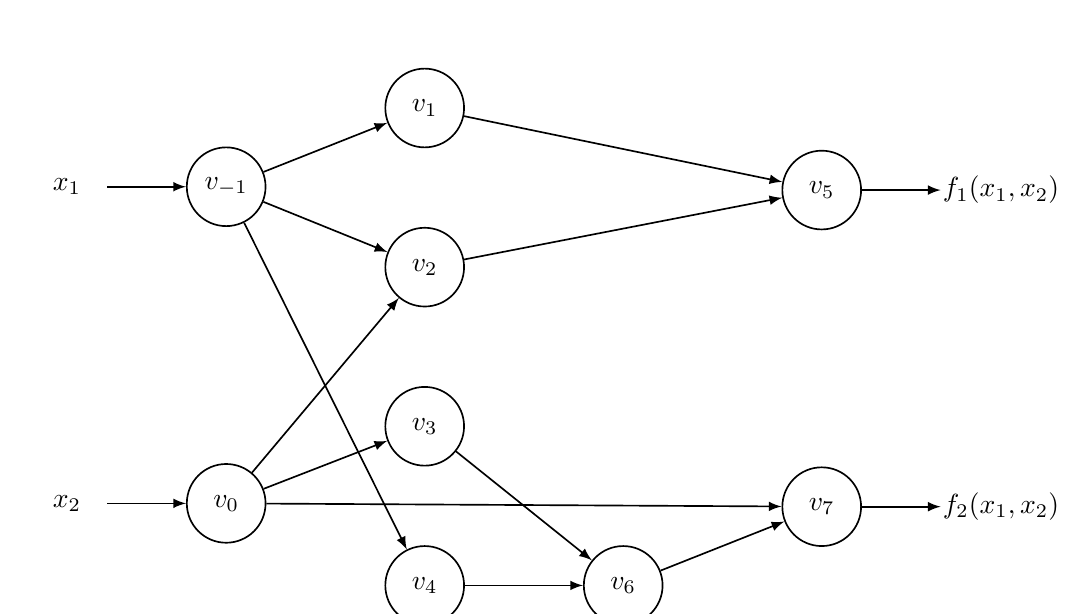
\begin{tikzpicture}
	[circle, inner sep=0pt, minimum size=10mm,
	operation/.style={draw},
	input/.style={draw=none},
	output/.style={draw=none}, -latex, auto, semithick]
	
	
	\node[operation] (v_minus_one) 				   								   {$v_{-1}$};
	\node[operation] (v_zero)	   [below=of v_minus_one, yshift=-20mm] 		   {$v_0$};
	\node[input]	 (x_one)	   [left=of v_minus_one] 						   {$x_1$};
	\node[input]	 (x_two)	   [left=of v_zero] 							   {$x_2$};
	
	\node[operation] (v_one)       [right=of v_minus_one, xshift=5mm, yshift=10mm] {$v_1$};
	\node[operation] (v_two)       [below=of v_one] 							   {$v_2$};
	\node[operation] (v_three)     [below=of v_two] 							   {$v_3$};
	\node[operation] (v_four)      [below=of v_three] 							   {$v_4$};
	
	\node[operation] (v_six)       [right=of v_four, xshift=5mm] 				   {$v_6$};
	
	\node[operation] (v_seven)     [right=of v_six, xshift=5mm, yshift=10mm] 	   {$v_7$};
	\node[operation] (v_five)      [above=of v_seven, yshift=20mm] 			   	   {$v_5$};
	\node[output]	 (f_one)	   [right=of v_five] 							   {$f_1(x_1,x_2)$};
	\node[output]	 (f_two)	   [right=of v_seven] 							   {$f_2(x_1,x_2)$};
	
	
	\draw [->] (x_one)		 to (v_minus_one);
	\draw [->] (x_two)		 to (v_zero);
	\draw [->] (v_minus_one) to (v_one);
	\draw [->] (v_minus_one) to (v_two);
	\draw [->] (v_minus_one) to (v_four);
	\draw [->] (v_zero) 	 to (v_two);
	\draw [->] (v_zero) 	 to (v_three);
	\draw [->] (v_zero) 	 to (v_seven);
	\draw [->] (v_one)		 to (v_five);
	\draw [->] (v_two)		 to (v_five);
	\draw [->] (v_three)	 to (v_six);
	\draw [->] (v_four)	 	 to (v_six);
	\draw [->] (v_six)		 to (v_seven);
	\draw [->] (v_five)		 to (f_one);
	\draw [->] (v_seven)	 to (f_two);
\end{tikzpicture}
\caption{Computational graph of function $\tilde{f}(x_1, x_2) = \Bigl[
		\tilde{f}_1(x_1, x_2) \,\, \tilde{f}_2(x_1, x_2) \Bigr]$. Definitions of intermediate variables $ v_{-1}, \dots, v_7$ are given in table~\ref{tab:forward_AD_example} or~\ref{tab:backward_AD_example}}
\label{fig:example_of_computational_graph}
\end{figure}

Using the aforementioned representations we see that every function ultimately is a composition of elementary operations. This also means that its numerical derivatives can be computed by combining all the numerical derivatives of the constituent operations through the \emph{chain rule}: this, is the main idea of AD.

%TODO: 1) Talk about automatic label misconception
%Before going ahead we would like to draw reader's attention on the risk of ambiguity that the term ``automatic'' in  AD generate. One might label as AD every technique that allows to compute derivatives without computing them manually (e.g. Symbolic Differentiation), but in technical terms AD is used to indicate only those techniques that compute derivatives through accumulation of values during code execution to generate numerical numerical derivative evaluations rather than derivative expression.

%TODO: 2) Talk about that AD work also with regular code constructs
%We also emphasize the advantage of AD that can be applied to regular code with minimal change, allowing branching, loops and recursion unlike manual and symbolic differentiation which require to arrange the code under the syntactic and semantic constraint of the obtained formulas.


\subsection{Forward mode}

In order to compute the derivative of the function $\tilde{f}$, reported in~\eqref{eqn:example_function_for_AD}, respect to $x_1$ we start by considering the evaluation trace on the left-hand side of table~\ref{tab:forward_AD_example} and we associate to each intermediate variable $ v_i$ the derivative:
\[
	v_i' = \frac{\partial v_i}{\partial x_1}
\]
Moving from top to bottom in the forward primal trace the corresponding tangent (derivative) trace, presented on the right-hand side of table~\ref{tab:forward_AD_example}, is generated by applying the chain rule to each encountered operation. After the primals $v_i$ are evaluated, also the corresponding tangents $v_i'$ are, again, from top to bottom; this gives us the desired derivatives in the final variables $v_5' = \frac{\partial y_1}{\partial x_1}$ and $v_7' = \frac{\partial y_2}{\partial x_1}$.
%One of the advantages using this implementation is that, in just one forward pass, we obtained all the derivatives respect $x_1$.

\medskip
Forward mode can also be employed to evaluate the Jacobian of a generic function $f \colon \R^n \to \R^m$ at a point $\vec{x} = \vec{a}$ by performing $n$ distinct forward passes. By setting only one variable $x_i'=1$ and the others to zero we obtain:
\[
	y_j' = \frac{\partial y_j}{\partial x_i}\bigg|_{\vec{x}=\vec{a}} \qquad j=1,\dots,m.
\]
and reiterating for $ i=1,\dots,n$, placing the resulting vectors side by side, we eventually obtain the Jacobian of $f$:
\[
\vec{J}_f =
\left.
\begin{bmatrix}
	\frac{\partial y_1}{\partial x_1} &  \dots  & \frac{\partial y_1}{\partial x_n}  \\
	\vdots							  & \ddots  & \vdots							 \\
	\frac{\partial y_m}{\partial x_n} &  \dots  & \frac{\partial y_m}{\partial x_n}
\end{bmatrix}
\right|_{\vec{x} = \vec{a}}
\]

Furthermore, by properly fine-tuning the values of the variables $x_1', \dots, x_n'$ is possible computing efficiently and in a matrix-free way Jacobian-vector products:
\[
\vec{J}_f \vec{r} =
\begin{bmatrix}
	\frac{\partial y_1}{\partial x_1} &  \dots  & \frac{\partial y_1}{\partial x_n}  \\
	\vdots							  & \ddots  & \vdots							 \\
	\frac{\partial y_m}{\partial x_n} &  \dots  & \frac{\partial y_m}{\partial x_n}
\end{bmatrix}
\begin{bmatrix}
	r_1		\\
	\vdots  \\
	r_n
\end{bmatrix}
\]
To accomplish this all that needs to be done is simply initializing $\vec{x}'=\big[x_1', \dots, x_n' \big]$ with $\vec{r}$; this result is particularly important in the evaluation of directional derivatives.
Before moving on, it is crucial to point out that forward mode AD:
\begin{itemize}
	\item for a function $f \colon \R \to \R^m$ allows to evaluate all its derivatives in just one forward pass, regardless of $m$;
	\item for a scalar field $f \colon \R^n \to \R$, the evaluation of its gradient $\nabla f = \Bigl[ \frac{\partial y}{\partial x_1}, \dots, \frac{\partial y}{\partial x_n} \Bigr]$ always require $n$ evaluations (since gradient is nothing more than a Jacobian of size $1 \times n$).
	%TODO: Add note of the factthat that it is not advantageous respect others methods
\end{itemize}
This means that the here explained implementation of AD is effective during the computation of derivative for cases $f \colon \R^n \to \R^m$ where $n \ll m$. For cases $n \gg m$ \emph{reverse mode} is more beneficial; we will discover why in the following subsection.

\begin{table}
\centering
	\begin{tabular}{cll}
		\toprule
		\multicolumn{3}{l}{\text{Forward Primal Trace}}  	 \\
		$v_{-1}$ &  $=x_1$ 				  & $=2$  			 \\
		$v_0$	 &  $=x_2$ 				  & $=3$  			 \\
		\midrule
		$v_1$	 &  $=\cos v_{-1}$  	  & $=\cos 2$      	 \\
		$v_2$	 &  $=v_{-1}  v_0$  	  & $=2 \cdot 3$  	 \\
		$v_3$	 &  $=v_0^3$  			  & $=3^3$	  	  	 \\
		$v_4$	 &  $=\ln v_{-1}$  	  	  & $=\ln 2$  	  	 \\
		$v_5$	 &  $=v_2 + v_1 \quad$    & $=6-0.416$   	 \\
		$v_6$	 &  $=v_3 + v_4$  		  & $=27+0.693$  	 \\
		$v_7$	 &  $=v_6 - v_0$  		  & $=27.693-3$  	 \\
		\midrule
		$y_1$	 &  $=v_5$				  & $=5.584$		 \\
		$y_2$	 &  $=v_7$				  & $=24.693$		 \\
		\bottomrule
	\end{tabular}
%	\begingroup\setlength{\fboxsep}{0pt}
%	\colorbox{lightgray}{
		\begin{tabular}{cll}
			\toprule
			\multicolumn{3}{l}{\text{Forward Tangent (Derivative) Mode}}  							 \\
			$v'_{-1}$ 		 &  $=x'_1$						  			& $=1$  					 \\
			$v'_0$	  		 &  $=x'_2$ 					  			& $=0$  					 \\
			\midrule
			$v_1'$	  		 &  $=-v_{-1}'\sin v_{-1}$  	  			& $= -\sin 2 \cdot 1$      	 \\
			$v_2'$	  		 &  $=v_{-1}'  v_0 + v_{-1}  v_0' \quad$	& $=1 \cdot 3 + 2 \cdot 0$ 	 \\
			$v_3'$	  		 &  $=3  v_o^2  v_0'$  						& $=3 \cdot 2^2 \cdot 0$  	 \\
			$v_4'$	  		 &  $=v_{-1}' / v_{-1}$  			  		& $=1/2$	  	  	 		 \\
			$v_5'$	  		 &  $=v_2' + v_1'$  		  				& $=3 - 0.909$   	 		 \\
			$v_6'$	  		 &  $=v_3' + v_4'$  		  				& $=0+0.5$  	  			 \\
			$v_7'$	  		 &  $=v_6' - v_0'$  		  				& $=0.5 - 0$  				 \\
			\midrule
			$\mathbf{y'_1}$	 &  $\mathbf{=v_5'}$				  		& $\mathbf{=2.091}$			 \\
			$\mathbf{y'_2}$	 &  $\mathbf{=v_7'}$				  		& $\mathbf{=0.5}$			 \\
			\bottomrule
		\end{tabular}
%	} \endgroup
\caption{Forward mode AD example to evaluate the derivatives $\frac{\partial y_1}{\partial x_1}$ and $\frac{\partial y_2}{\partial x_1}$ of $\tilde{f}(x_1, x_2)$ at $[x_1, x_2] = [2,3]$. $x_1'$ and $x_2'$ are respectively set to $1$ and $0$ in order to derive only respect $x_1$. On the left is reported the forward evaluation trace, on the right the tangent one}
\label{tab:forward_AD_example}
\end{table}

%TODO: 1) Aggiungi colore alla tabella di dx
%TODO: 2) Aggiungi descrizione tabelle
%TODO: 3) Aggiungi frecce alle tabelle





\subsection{Reverse mode}

\section{Adjoint method}
%TODO 1: cos'è e come funziona in generale

Come viene applicato in generale


Come viene applicato il metodo dell'aggiunto nel metodo RBF-FD


























\chapter{Results}

\section{Poisson Equation}
\label{sec:poisson_equation}

Given a region $\Omega \subset \R^d$, with $d \in \N$ and bounded by the boundary $\partial\Omega$, the generic heat equation with internal heat generation~\cite{Brezis:functional_analysis_book}, at steady state, is described by the Poisson Equation which is defined by the following Partial Differential Equation (PDE):
\begin{equation}
	\label{eqn:Poisson_equation}
	\begin{cases}
		- \Delta u(\vec{x}) = q(\vec{x})														 &  \text{in $\Omega$}							\\
		\mathcal{B} u(\vec{x}) = g(\vec{x})  																		&  \text{on $\partial\Omega$}
	\end{cases}
\end{equation}
where $\Delta$ indicates the Laplacian operator, $\mathcal{B}$ is the (possibly differential) linear operator that enforce the boundary conditions (BCs) and $q$ and $g$ are known functions. Clearly Poisson Equation is one of the many PDE that can be solved using meshless methods, including the RBF-FD discussed in this thesis.

We decided to evaluate the results of the adjoint method applied to RBF-FD method on the aforementioned equation due to both its wide range of applications in different areas	(e.g. electrostatic, chemistry, gravitation and others) and the simplicity of its analytical manipulation.

In particular for this thesis and to obtain the results presented in this chapter we implemented RBF-FD method as follow:
\begin{itemize}
%TODO: 	\item consider domains $\Omega \subset \R^{d}$ with $d=1,3$;  Da spostare nell'intro ai results
	\item use RBFs augmented with polynomial terms as basis functions $B_k$ to approximate the solution $u$ in a similar way to what has been done in~\cite{Liu:Intro_to_meshfree_methods}; 
	\item formulate the problem in its strong form, so we will use the collocation technique in combination with the Weighted Residual Method.
\end{itemize}
thus we will apply the RBF-generated Finite Differences (RBF-FD)~\cite{Fornberg:RBF-FD_1, Fornberg:RBF-FD_2} to solve~\eqref{eqn:Poisson_equation} in one and three dimensional physics domain.
% "Collocation methods with Weighted Residual Methods" Cioè prima hai citato i collocation, ma i weighted residual da dove saltano fuori?? Da spiegare meglio/togliere??

Mono dimensional physics domain are used to gain confidence with the techniques explained while three dimensional  domain are used for their application in real case problems as those faced at Esteco. $2$D cases, instead, have been skipped in the analysis since they would only be used to bridge the 2 previous scenarios and therefore would have had no practical utility.

RBFs are used for scattered data interpolation both for their physical foundation[overview 20, Hardy 1990] and for their profitable use in applications like meteorology, turbulence analysis and neural network~\cite{Chen:meshless_overview_after_20_years}

Finally, collocation technique is employed because thanks to its ability to discretize the Boundary Value problem~\eqref{eqn:Poisson_equation} expressed in strong form leads to a real fully meshless approach~\cite{Miotti:RBF_in_depth}.


\section{1D case}

In this case $d=1$, the physical domain is simply a segment and its boundary consists on its two endpoints that we indicate with $a$ and $b$, both belonging to $\R$. Therefore we have $\Omega =~]a,b[$ and $\partial\Omega = \Set{a, b}$.
With respect to the rest of the boundary value problem we define $q(x) = - \omega^2 \sin(x)$ and we impose the following Dirichlet BCs: $u(a)=q(a)$ and $u(b)=q(b)$. Fixing the values $\omega=1$, $a=0$ and $b=\pi$ allows to rewrite the Poisson equation reported in~\eqref{eqn:Poisson_equation} as
\begin{equation}
	\label{eqn:Poisson_equation_1D}
	\begin{cases}
		- \Delta u(\vec{x}) = - \sin(x)  &  \text{in $]a,b[$}  \\
		u(a) &= 0  \\
		u(b) &= 0
	\end{cases}
\end{equation}
In order to find an approximated solution to the problem~\eqref{eqn:Poisson_equation_1D} we employ the RBF-FD method parametrized as follow:
\begin{itemize}
	\item $\varphi(r) = r^3$ Polyharmonic function is used as basic function to define the RBF interpolant;
	\item $P=2$ is the degree of its polynomial augmentation;
	\item $N=41$ evenly spaced nodes are used for domain discretization: $N_I=39$ are placed in $\Omega$ and the other $N_B=2$ are placed repsectivelly in $a$ and $b$;
	\item $m=7$ is the number of nodes which constitute a single stencil;
\end{itemize}
As done previously we indicate with $\vec{u}_I$ the vector obtained by solving the system~\eqref{eqn:compact_discretized_PDE} derived from RBF-FD discretization.
%TODO: Sposta il vincolo dopo la cost function
The discretized version Equation~\eqref{eqn:Poisson_equation_1D} will be the constraints during the optimization

The design optimization problem, related to segment $[a,b]$, that we want to solve is the minimization of the following cost function:
\begin{equation}
	J(\vec{u}_I, b) = \frac{1}{2} \frac{b}{N-1} \left( \sum_{i=2}^{40} u(x_i) - E \right)^2
\end{equation}
where $\vec{u}_I$ is the result of the 
where it can be seen the single design variable, $l=b$ and the result of th esingle  which means that in order to meet the objective we are allowed to vary the length of the segment $[a,b]$.
The discretized version Equation~\eqref{eqn:Poisson_equation_1D} will be the constraints during the optimization

The results after $30$ steps in the optimization procedure are shown in figure~\ref{fig:opt_results_1D}.

\begin{figure}
	\centering
	\includegraphics[width=.75\textwidth]{img/uOpt_vs_x_1D.pdf}
	\caption{discretized approximated solution obtained solving~\eqref{eqn:Poisson_equation_1D} via RBF-FD at the end of the design optimization. $b_0$ and $b_{30}$ indicate respectively the intial and the final position of the $b$ endpoint}
	\label{fig:opt_results_1D}
\end{figure}

while in figure~\ref{fig:opt_history_1D} are shown the dynamic of the cost function and of its gradient respect the design variable $b$.

\begin{figure}
	\centering
	\subfloat[][\emph{Cost function values}]
		{\includegraphics[width=.45\textwidth]{img/cost_vs_iter_1D.pdf}} \quad
	\subfloat[][\emph{Cost function gradient values}]
		{\includegraphics[width=.45\textwidth]{img/costGrad_vs_iter_1D.pdf}}
	\caption{Trajectories of the cost function and its gradient throughout the optimization process}
	\label{fig:opt_history_1D}
\end{figure}

In this case we would like to modify the 
For the experiments we initially imposed $a=0$ and $b=\pi$.
In this case we have only one design parameter $l$ that let modify the shape of the physical domain and it is the position of the endpoint $b$. The whole  system can be thought as a bar whose length can be varied.



\section{3D case}

%*******************************************************
% Conclusion
%*******************************************************
\chapter*{Conclusion}
% Do not edit
\addcontentsline{toc}{chapter}{Conclusion}
\label{chap:concl}
\markboth{CONCLUSION}{CONCLUSION}

\lipsum[1]

\section{Lorem Ipsum}
\lipsum[2-4]

\subsection{Dolor sit amet}
\lipsum[5-7]

%*******************************************************
% Appendix
%*******************************************************
% Do not edit
\pagestyle{fancy}
\renewcommand{\chaptermark}[1]{\markboth{\MakeUppercase{APPENDIX\ \thechapter.\ #1}}{}}

\appendix
\label{appendix}

\chapter{Stereolithography \texttt{.stl} files}

\verb|.stl| is a file format which dates back to $1987$ when it has been created by \textit{$3$D Systems}\footnote{American company that engineers, manufactures and sells $3$D printers, $3$D printing materials, $3$D printed parts and application engineering services. For further information we refer to~\url{https://www.3dsystems.com/}} for its stereolithography (from which the file extension originates) printing technology for commercial $3$D printers. Eventually it became the $3$D printing and rapid prototyping industry's defacto standard. In general \verb|.stl| files are also referred to as standard triangle language or standard tessellation language files.

\smallskip
The \verb|.stl| format is used to describe an unstructured triangulated surface using a list of triangles. Each of these triangles is described separately by its own normal and  vertices using a Cartesian coordinate system~\cite{wiki:stl_file_format}. Their main purpose is to describe the surface geometry of a $3$D object, thus in this files, differently from CAD files, no information about colors or textures is present. They also do not contain any scale information and can be specified both in ASCII and binary representation.

\smallskip
An example of of a \verb|.stl| file in ASCII format is:
\begin{verbatim}
solid topFace
    facet normal -0.000000e+00  0.000000e+00  1.000000e+00
        outer loop
            vertex   0.000000e+00 -0.000000e+00  5.000000e-01
            vertex   5.000001e-02 -5.000001e-02  5.000000e-01
            vertex   5.000001e-02 -0.000000e+00  5.000000e-01
    endloop
endfacet
...
endsolid topFace
solid fixedFaces
    facet normal  0.000000e+00  1.000000e+00  0.000000e+00
        outer loop
            vertex   0.000000e+00 -0.000000e+00  0.000000e+00
            vertex   5.000001e-02 -0.000000e+00  5.000000e-02
            vertex   5.000001e-02 -0.000000e+00  0.000000e+00
        endloop
    endfacet
...
endsolid fixedFaces
\end{verbatim}
This is the \verb|.stl| file that we have used to represent the geometry used in the $3$D design optimization problem in section~\vref{sec:results_3D_case}. In the same file showed above are stored two different surfaces named respectively \verb|topFace| and \verb|fixedFaces|; each triangle of a surface is described by means of a \verb|facet| (we reported only one triangle per surface for brevity) which specify its normal and the coordinates of its vertices arranged counterclockwise.
Those files can also be stored in binary format, which is particularly convenient for large files.

\smallskip
We finally remark that, in general, \verb|.stl| files contain only an \emph{approximation} of geometry surfaces. An example of this situation can be found in figure~\vref{fig:sphere_real_and_meshed}, specifically in figure~\ref{subfig:sphere_meshed} it can be seen how the red lines of the triangle edges are not capable to perfectly reconstruct the smoothness of the original surface (figure~\ref{subfig:sphere_real}). Augmenting the number of triangles of the mesh improve the approximation, at cost of larger \verb|.stl| files, but will not be possible to perfectly reconstruct curved surfaces.

\begin{figure}
	\centering
	\subfloat[][\emph{Original sphere}]
	{\includegraphics[width=.55\textwidth]{img/sphere_real.png}\label{subfig:sphere_real}} \\
	\subfloat[][\emph{Sphere \texttt{.stl} representation}]
	{\includegraphics[width=.55\textwidth]{img/sphere_meshed.png}\label{subfig:sphere_meshed}}
	\caption{Example of approximating the surface of a unit-radius sphere centered at the origin using an \texttt{.stl} file}
	\label{fig:sphere_real_and_meshed}
\end{figure}

%TODO: About the history


\backmatter

%*******************************************************
% Bibliography
%*******************************************************
\nocite{*}
\printbibliography

%*******************************************************
% FinalDedication
%*******************************************************
% Do not edit
\chapter*{}
\thispagestyle{empty}
\vspace*{3cm}

\begin{center}
\hfill Ei fu. Siccome immobile, \\
\hfill Dato il mortal sospiro, \\
\hfill Stette la spoglia immemore \\
\hfill Orba di tanto spiro \\ \medskip
\hfill Alessandro Manzoni -- \emph{Il Cinque Maggio}
\end{center}

\end{document}